
\documentclass{article}
\usepackage[utf8]{inputenc}
\usepackage{blindtext}
\usepackage{graphicx}
\usepackage{amsmath}
\usepackage{csvsimple}
\usepackage{pdfpages}
\usepackage{hyperref}
\usepackage{gensymb}

\begin{document}
\begin{center}
\textbf{\Huge{University of South Bohemia}}\\
\vspace{50px}
\textbf{\Large{Faculty of Science}} \\
\vspace{30px}
\includegraphics[width=120px]{~/school/logo.png} \\
\vspace{30px}
\textbf{\large{Praktika IV}}
\vspace{20px}
\\
\vspace{20px}
\large{Rutherfordův experiment} \\
\vspace{60px}
\end{center}
\begin{flushleft}
Datum: 24.10.2023 \\
Jmeno: Martin Skok \\
Obor: Fyzika \\
Hodnoceni:
\end{flushleft}
\newpage
\section{Úkoly}
Změřte závislost počtu rozptýlených $\alpha$ částic na úhlu rozptylu
\section{Pomůcky}
Experimentální komora, zdroj $\alpha$ částic $^{241}A_{m}$, pumpa na vysátí vzduchu, hadičky, čítač.
\section{Teorie}
Rutherfordův experiment potvrdil, že v atomu existuje jádro a vyvrátil Thompsonovu teorii.
Rutherfordův rozptyl popisuje interakci mezi nabitými částicemi a jejich rozptylem, většinou se bavíme o alfa částici a jádru. Když alfa částice přiletí k jádru atomu, bude na ní působit coloumbovská síla, která způsobí, že částice bude odpuzováná a rozptýlena pod nějakým úhlem. Ná částici působí i další síly, ale ty zanedbáváme, protože jsou velmi malé.
Pro detektor pod určitým úhlem vzhledem k dopadajícímu paprsku je počet částic na jednotku plochy dopadajících na detektor dán Rutherfordovým vzorcem:
\begin{equation}
  N(\theta) = \frac{N_{i}n L Z^{2} k^{2} e^{4}}{4 r^{2} K E^{2} sin^{4}(\frac{\theta}{2})}
\end{equation}
Kde $N_{i}$ je počet dopadajících alfa částic,
$n$ je atom na jednotku objemu v destičce,
$L$ je šířka destičky,
$Z$ je atomové číslo destičky,
$e$ je náboj elektronu,
$k$ je coloumbova konstanta,
$r$ je vzdálenost mezi detektorem a destičkou,
$KE$ je kinetická energie alfa částice,
$\theta$ je úhel rozptylu
\begin{figure}[h]
  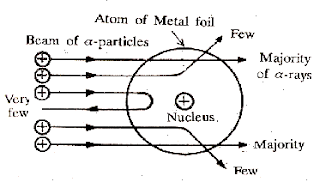
\includegraphics[scale=0.8]{data/ruther.png}
  \caption{Rutherfordův rozptyl}
\end{figure}
\section{Postup měření}
Můj vedoucí praktik zapnul měřák dávkového příkonu Radigem.
Do komory jsem vložil vzorek.
Měřící komoru jsem připojil k pumpě, aby jsem z ní mohl vysát vzduch a vytvořit vakuum.
Ke komoře jsem připojil k čítači, který ukazoval počet detekovaných částic.
Zapnul jsem čítač a nastavil ho do polohy $N_{A_E}$.
Rameno se vzorkem jsem otočil do polohy 30°, aby na detektor dopadalo minimální množství částic.
Zapnul jsem čítač a postupně zvyšoval diskriminační napětí, kdy šum klesl na nulovou hodnotu.
Zaznamenal jsem si hodnotu.
To samé jsem udělal pro úhel 0° a zaznamenal jsem si hodnotu.
Diskriminační napětí jsem potom nastavil na střed těchto hodnot.
Pomocí tlačítka GATE jsem nastavil čas na 100 sekund a měřil jsem četnost částic pro úhly 0° 5° -5° 10° -10° 15° -15°.
Podobně jsem měřil pro úhly 20° -20° (200s), 25° -25° (600s) a 30° -30° (900s).
\newpage
\section{Zpracování dat}
\footnotesize{Tabulka 1}\\
\csvreader[
tabular = |c|c|c|c|,
table head =
\hline
{Úhel $\theta$} & {počet částic $n$} & {čas $t[s]$} & {četnost částic $N$}\\
\hline
\hline,
late after line = \\\hline
]{data/data1.csv}{}{
  \csvcoli & \csvcolii & \csvcoliii & \csvcoliv}
\\
\vspace{1em}
\\
$N$ je počítáno jako $\frac{n}{t}$.\\
Data jsem vynesl na graf spolu se křivkou následujícího tvaru, kterou pojmenuju $f(\theta)$
$$f(\theta) = \frac{A}{sin^{4}(\frac{\theta - B}{2})}$$
jedná se o rovnici 1, ale všechny konstanty jsem nahradil jednou a pojmenoval jsem ji $A$.
Konstanta $B$ je pak vertikální posun.
\newpage
\begin{figure}[!h]
  \hspace*{-5em}
  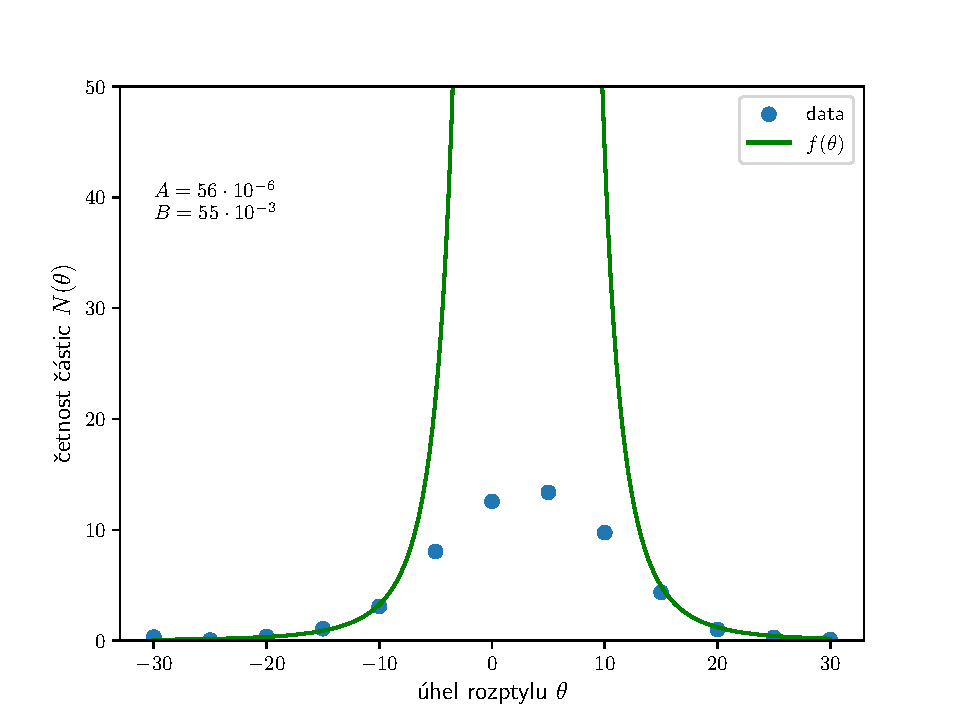
\includegraphics[scale=0.8]{data/graph1.pdf}
  \caption{Závislost četnosti částic $N(\theta)$ na úhlu $\theta$}
\end{figure}
\section{Diskuse}
Při zpracování dat, jsem hledal konstanty A a B od oka.
Mohl jsem možná použít jiné matematické metody, jako Lagrangeovi multiplikátory,
ale na tuhle úlohu by to bylo až moc zbytečné složité.
Když budu vycházet z rovnice 1, znamená to, že naměřená konstanta A je
$$A = \frac{N_{i}n L Z^{2} k^{2} e^{4}}{4 r^{2} K E^{2}}$$
\section{Závěr}
$$A = 56 \cdot 10^{-6}$$
$$B = 55 \cdot 10^{-3}$$
\section{Zdroje}
\url{http://hyperphysics.phy-astr.gsu.edu/hbase/rutsca.html}
\end{document}
